\documentclass[11pt, class=article, crop=false]{standalone}
\usepackage[subpreambles=true]{standalone}
\usepackage[T1]{fontenc} % for font setting
\usepackage{newtxtext,newtxmath}
\usepackage{import,
            graphicx,
            parskip,
            url,
            amsmath,
            wrapfig,
            fancyhdr,
            soul,
            tabularx,
            authblk,
            textcomp,
            lineno}

% side caption figure
\usepackage{sidecap}
\sidecaptionvpos{figure}{t}

% for special characters in bibliography            
\usepackage[utf8]{inputenc}
\usepackage[T1]{fontenc}

% citation setup
\usepackage[euler]{textgreek}
\usepackage[sort&compress]{natbib}
\setcitestyle{semicolon}
\bibliographystyle{bioconv}

% caption setup
\usepackage[font={f, small}, labelfont={bf, small}]{caption}
           
% color box
\usepackage[most]{tcolorbox}
\tcbuselibrary{breakable}

% margin
\usepackage[top=2.54cm, bottom=2.54cm, left=2.54cm, right=2.54cm]{geometry}%set margin

% title
\title{Restoration of aquatic habitat complex extends the foraging window of terrestrial consumers}
\date{} % remove date from title
\author{}

% % author list
% \author[1, a]{Mason Ibrahim}
% \author[2]{Radmila Petric}
% \author[1, b]{Charles F. Wahl}
% \author[1, *]{Akira Terui}

% \affil[1]{Department of Biology, University of North Carolina at Greensboro}
% \affil[2]{Institute for the Environment, University of North Carolina at Chapell Hill}
% \affil[a]{Current Affiliation: Nicholas School of the Environment, Duke University}
% \affil[b]{Current Affiliation: Colorado Water Science Center, U. S. Geological Survey}
% \affil[*]{Corresponding Author: hanabi0111\@gmail.com}

\linenumbers

\begin{document}

\maketitle

\section*{Abstract}

Cross-ecosystem linkages benefit generalist consumers by providing prey fluxes from donor habitats, but these trophic connections are highly vulnerable to human influences.
Evidence shows that restoring degraded habitats can re-establish these linkages; however, the potential interaction between restored and remnant donor habitats remains poorly understood.  
Here, we show that constructed wetlands synergize with adjacent remnant streams by supplying spatial subsidies (emerging aquatic insects) asynchronously, effectively extending the foraging window for terrestrial consumers.
While stream insects primarily emerged in spring to early summer, constructed wetlands exhibited a distinct peak in mid-summer, creating resource waves that terrestrial consumers may exploit over an extended period.  
Indeed, increased bat activity was observed in a restored site with a constructed wetland adjacent to a remnant urban stream.
However, this positive effect diminished when a constructed wetland was located in a closed forest canopy area, where dense canopies may reduce prey accessibility for bats.
These findings illuminate the context-dependent synergy between restored and remnant habitats in sustaining cross-ecosystem linkages, highlighting the importance of spatial design in restoration projects.

\section{Introduction}

Ecosystems are not isolated from each other, but are permeable to fluxes of energy and nutrients.
The energy flux across ecosystem boundaries, called spatial subsidies, originates from a donor ecosystem and influences biodiversity within a recipient ecosystem \citep{polis_toward_1997}.
Spatial subsidies can occur through several vectors, both physical and biological.
Physical movements of subsidies are mediated passively by wind, runoff, and currents (e.g., fallen leaves), whereas biological movements can happen by predation or periodic life-history events that allow materials to move across habitat boundaries, such as the emergence of aquatic insects from water bodies \citep{polis_toward_1997, baxter_tangled_2005, schindler_subsidies_2017}.

While recipient consumers benefit significantly from spatial subsidies \citep{nakano_reciprocal_2001, takimoto_seasonal_2002, terui_stream_2018}, such trophic linkages are vulnerable to human influences \citep{paetzold_environmental_2011, kraus_cross-ecosystem_2014, schulz_review_2015, tonra_barriers_2016}. 
Coal mining exemplifies such scenarios, where the lasting impact of environmental pollution from abandoned mines reduced the emergence of aquatic insects and the abundance of predators in recipient riparian ecosystems that rely on these subsidies \citep{paetzold_environmental_2011}.
The loss of trophic connections between ecosystems can impact the functioning of the recipient ecosystem \citep{sato_nematomorph_2012, sato_stage-specific_2014, terui_stream_2018}, which underpins the plethora of ecosystem services \citep{cardinale_biodiversity_2012}.

An increasing body of evidence suggests that restoring degraded habitats can be a powerful approach to maintaining trophic linkages between ecosystems \citep{buckner_conserving_2018, kupilas_stable_2020}.
For example, Kupilas et al. \citeyearpar{kupilas_stable_2020} demonstrated river restoration improves aquatic-terrestrial linkages.
The study, conducted across eleven river restoration projects in Europe, revealed a higher contribution of aquatic prey to the riparian arthropod diet in restored river sections through stable isotope analysis.
These findings highlight the importance of habitat restoration in maintaining cross-ecosystem trophic interactions.

However, how restored habitats interact with the remnant donor habitats to sustain trophic linkages across ecosystems remains poorly understood.
Spatial subsidies arise from diverse donor habitats, each with unique temporal patterns of subsidy production \citep{schindler_portfolio_2015, schindler_subsidies_2017}.
For example, in environments with clear seasonality, the variation in thermal regimes among aquatic habitats leads to asynchronous seasonal peaks of spatial subsidies in space \citep{nash_latitudinal_2023}, broadening foraging opportunities for mobile consumers that track resource waves within a landscape \citep{schindler_riding_2013, ruff_temperature-associated_2011, armstrong_resource_2016}.
The extended foraging opportunity driven by phenological diversity is crucial for the long-term persistence of subsidized consumers, particularly in the face of environmental change \citep{fryxell_landscape_2005, armstrong_watershed_2020}.
Thus, habitat restoration may extend beyond simply substituting lost habitats; it may work in concert with remaining donor habitats to enhance cross-ecosystem trophic linkages.
The significance of such restoration efforts, however, may depend on the structural characteristics of the recipient ecosystem, where greater accessibility to spatial subsidies could enhance trophic transfer efficiency \citep{marczak_meta-analysis_2007, terui_species-specific_2017}.
These interacting factors likely influence the overall impact of habitat restoration on cross-ecosystem connections.

In this study, we examine the role of urban wetland restoration in supporting terrestrial consumers, such as bats, by improving cross-ecosystem trophic linkages.
Wetlands provide essential ecosystem services, including the provision of spatial subsidies to adjacent ecosystems \citep{schindler_subsidies_2017, reis_global_2017}.
With $\sim$25\% of the world’s wetlands lost since 1700's \citep{fluet-chouinard_extensive_2023}, there is a growing movement to restore these critical habitats \citep{reis_global_2017}.
We aim to test the following hypotheses, building on previous studies that have shown that adding constructed wetlands in urban areas can significantly increase the foraging activity of insectivorous bats \citep{parker_rapid_2019, li_four_2021}.
First, we hypothesize that remnant streams and constructed wetlands would exhibit asynchronous emergence of aquatic insects over the year, thereby providing bats with an extended foraging window. 
Second, we hypothesize that the landscape context of restored habitats may influence their effectiveness as subsidy sources for specific recipient species.
Specifically, we predicted that dense canopy cover may hinder bats' movement, impacting the effectiveness of wetland restoration for trophic connections in those areas.

\newpage

\section{Methods}

\subsection{Study System}

We conducted our investigation in Peabody Park, located on the University of North Carolina Greensboro (UNCG) campus ($36.0725^\circ$N, $79.8088^\circ$W), Greensboro, NC, USA.
UNCG is an urban campus, surrounded by residential areas.
Surveys were conducted at four sites within this urban landscape, comprising two pairs of restored and control sites.
The first pair of restored and control sites were located in a grassland habitat area with an open canopy.
Within this area, the restored site had a constructed wetland near an urban stream (open-restored; wetland and stream) and the control site had a corresponding control without a wetland (open-control; stream only).
The second pair of sites were located within the Peabody Park forest.
Similar to the open area, the restored site had a constructed wetland (closed-restored; wetland and stream) while another site represented a control without a wetland (closed-control; stream only).
In both areas, restored and control sites were separated by $<$ 500 m to align background environmental conditions between the two sites.
This sampling design helps minimize the influence of potential confounding factors.

The two wetlands were constructed in March 2017.
These are small in size ($< 1000~\text{m}^2$) and shallow ($\sim 0.5$ m in maximum depth). 
The open wetland supports emergent and submerged plants with clear water, whereas the closed wetland is constantly turbid and no emergent and submerged plants are established.
See Parker et al. \citeyear{parker_rapid_2019} for more details.

\subsection{Emerging Aquatic Insect}

We investigated the phenology of aquatic insect emergence at the two restored sites (open-restored and closed-restored), each encompassing a stream and a small constructed wetland in proximity ($\le$ 20 m apart).
Emergence phenology was not assessed at the two control sites, based on the assumption that their temporal patterns are similar to those of the adjacent restored sites.
We quantified insect emergence from wetlands and streams monthly from March 2021 to March 2022 by deploying dome-shaped emergence traps (0.25 m$^2$) for 2 -- 7 days (weather permitting) for each sampling event.
At each site, two emergence traps were deployed at each of the distinct aquatic habitats (i.e., wetland and stream), totaling four traps per site.
In the wetlands, the emergence traps were set on opposite sides of each other.
In the streams, the two emergence traps were set in a riffle and a pool to encompass habitat heterogeneity.
Trapped insects were navigated toward a collection bottle filled with 70\% ethanol.
After collecting the traps, the insects were counted, sorted by order (Ephemeroptera, Tricoptera, and Diptera; no Plecoptera was found), and then weighed to the nearest mg (wet weight).

\subsection{Bat Activity Survey}

We recorded bat activities at all four sites as described above.
The restored and control sites within each area can be assumed to be similar in other environmental conditions, including but not limited to terrestrial prey availability, site openness, and site accessibility for park visitors.
Therefore, this contrast allows us to quantify the influence of wetland restoration on bat activities while accounting for other environmental variables.

Using Song Meter SM4BAT-FS ultrasonic recorder and a SMM-U2 microphone suspended 8 m above the ground (Wildlife Acoustics Inc., Maynard, Massachusetts, USA), we recorded bat activity from sunset to sunrise nightly throughout the year.
Recorder maintenance was regularly performed (approximately every four to six weeks) to ensure batteries were changed and the devices were operational.
All audio files were downloaded during each maintenance event to an external hard-drive.  

All audio files were processed using Kaleidoscope (version 4.4, Wildlife Acoustics Inc., Maynard, Massachusetts, USA), to automatically identify bat passes to species, with automatic identification accuracy set to neutral.
Based on previous studies \citep{parker_rapid_2019, li_four_2021}, the following seven species were found in Greensboro and were therefore used as species identification references: \textit{Eptesicus fuscus} (Big brown bat), \textit{Lasiurus borealis} (Eastern red bat), \textit{Lasiurus cinereus} (Hoary bat), \textit{Lasionycteris noctivagans} (Silver haired bat), \textit{Nycticeius humeralis} (Evening bat), \textit{Perimyotis subflavus} (Tricolored bat), and \textit{Tadarida brasiliensis} (Mexican free-tailed bat).

A bat pass was defined as a recording that included a minimum of three complete bat echolocation call pulses within 0.5 seconds.
Additionally, we used the bat pass match ratio of 0.60 or greater to accept the species identification.
This is the minimum criterion for accurate species identification generated by comparing results between automatic and manual identification results.
If the conditions were not met, the bat passes were classified as ``no ID''. 
We defined bat activity as the total amount of bat passes, including both identified and non-identified bat passes.
Although total bat activity does not directly equate to foraging activity, the two are likely positively correlated, especially during biologically active periods of the year.

\subsection{Statistical Analysis}

% \subsubsection{Emergence Flux}

One goal of our study is to investigate how different aquatic habitats contribute to the temporal stability of aquatic insect emergence flux.
To quantify temporal instability, we used the coefficient of variation (CV), defined as the ratio of the temporal standard deviation to the mean.
We estimated the CV for the combined emergence flux across wetland and stream habitats at each site, referring to this value as the ``observed'' CV. 
We also derived a ``predicted'' CV, representing a weighted mean of the CVs calculated separately for each habitat.
Specifically, we estimated the predicted CV ($\mbox{CV}_p$) as:

\begin{equation}
    \mbox{CV}_p = p_w \mbox{CV}_w + (1 - p_w) \mbox{CV}_s,
\end{equation}

where $p_w$ is the proportional contribution of the wetland to the total emergence flux at a site, and $\mbox{CV}_w$ and $\mbox{CV}_s$ denote the CVs of emergence flux for the wetland and stream habitats, respectively. 
The predicted CV reflects the expected temporal variability assuming perfect synchronization of emergence fluxes across habitats \citep{thibaut_understanding_2013, moore_lifehistory_2014}.
A reduction in the observed CV relative to the predicted CV would indicate enhanced stability in resource supply beyond that expected from a single habitat type alone \citep{thibaut_understanding_2013, moore_lifehistory_2014}.
In this analysis, we used data collected from March to October, as insect emergence during the winter months was minimal.

While the temporal CV provides insights into variability in insect emergence, it does not explicitly capture seasonality. 
To address this, we also calculated circular statistics \citep{nash_latitudinal_2023, staggemeier_circular_2020}.
Specifically, we converted the months of emergence into angles on a unit circle to appropriately reflect the cyclical nature of seasons: January through October corresponded to angles from $0^\circ$ to $315^\circ$ in $45^\circ$ increments.
We sampled a vector of angle values proportional to monthly emergence flux (wet mass) to approximate the temporal patterns of emergence.
Then, using the R package \textit{circular} \citep{circular}, we calculated the seasonality metric $\rho$, which quantifies the degree of temporal clustering around the mean angle.
Values of $\rho$ range from 0 (no seasonality) to 1 (strong seasonality).
As with CV, we calculated $\rho$ for total emergence flux across wetland and stream habitats and compared these values with the predicted values.
This comparison allows us to document how the degree of seasonality in insect emergence changes when stream and wetland habitats are combined.

We employed a generalized additive model (GAM) to assess the effects of wetland restoration and site openness on bat activity.
We used bat activity data collected daily from March 1, 2021, to October 31, 2021, aligning with the emergence phenology of aquatic insects (see Results).
We assumed the daily bat detection count $y_i$ for observation $i$ followed a negative binomial distribution, where the expected value $\mu_i$ was linked to linear predictors and a smooth function as follows:


\begin{align}
    y_i &\sim \mbox{NB}(\mu_i, \theta), \nonumber\\
    \ln \mu_i &= \beta_0 + \sum_k \beta_k x_{k,i} + f(\mbox{Julian}_i)z_i.
\end{align}

$\beta_0$ and $\beta_k$ are the intercept and regression coefficients for linear predictors $x_{k,i}$ and $\theta$ is the dispersion parameter of the negative binomial distribution.
The term $f(\mbox{Julian}_i)z_i$ accounts for the site-specific seasonality, where $f(\mbox{Julian}_i)$ is a smooth function for the Julian date and $z_i$ is a dummy variable discerning a unique combination of site openness (closed vs. open) and restoration status (stream only vs. wetland and stream).

Our primary interest in the bat analysis is the contrast between the restored (wetland and stream) and control sites (stream only), and its contingency on the site openness.
Therefore, we included the site openness (close = 0, open = 1), restoration status (stream only = 0, wetland and stream = 1), and their interaction as linear predictors in the model.
It is important to note that these linear effects are estimated after accounting for the seasonality \textit{via} the smooth function $f(\mbox{Julian}_i)z_i$.

All statistical analysis was conducted in R version 4.3.2 \citep{r_program}. We used R package \textit{mgcv} to implement the GAM \citep{mgcv}.

\newpage

\section{Results}

\subsection{Temporal Patterns of Aquatic Insect Emergence}

The average emergence flux was generally comparable across areas and aquatic habitats, with the highest flux observed in the stream within the closed area (Figure \ref{fig:insect-phenology} and Table \ref{tab:emg}).
However, taxonomic compositions varied considerably.
Diptera dominated the emergence flux from wetlands (proportional contribution = 0.94), while Trichoptera (0.01) and Ephemeroptera (0.05) were present in negligible amounts.
In streams, Diptera also contributed substantially to total emergence flux (0.54), but here the proportion of Trichoptera was significant (0.46).
Ephemeroptera was present but rare in streams (< 0.01).

\begin{figure}
    \centering
    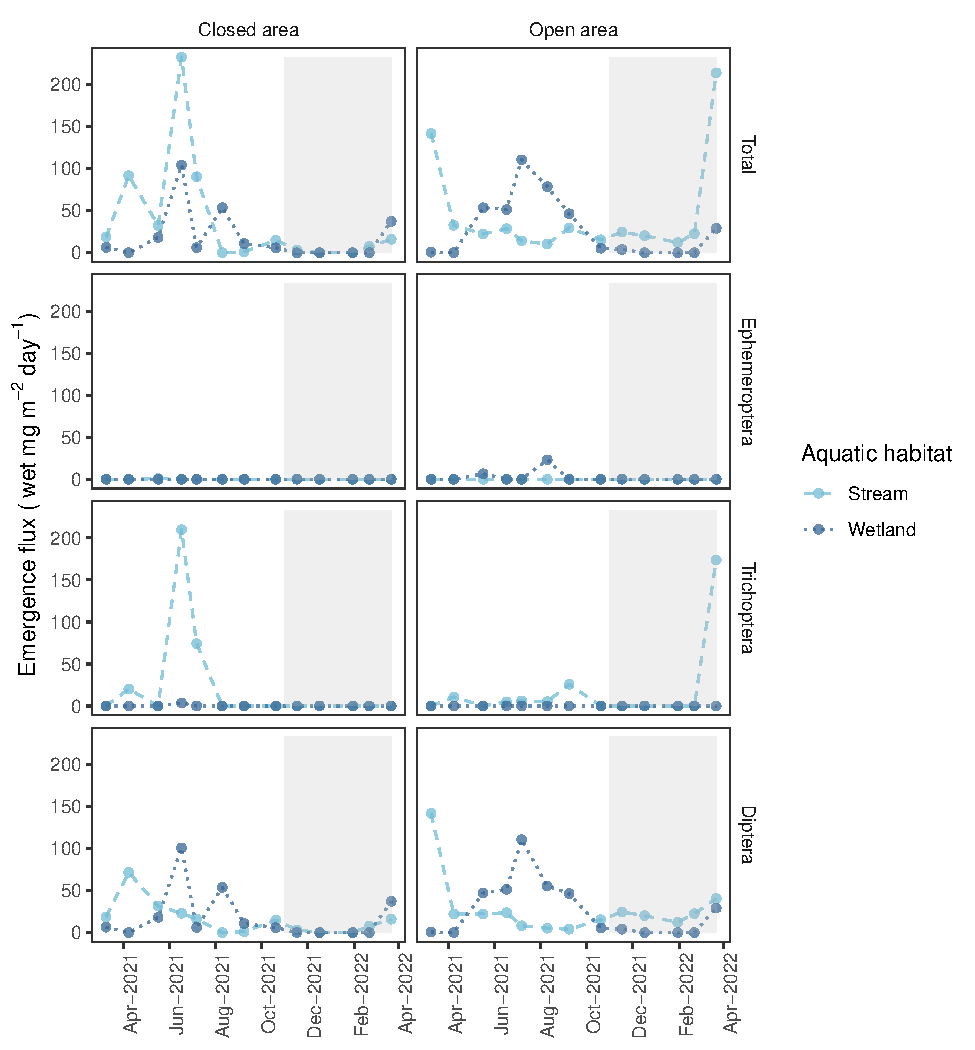
\includegraphics[width=0.75\textwidth]{output/figure_emg.pdf}
    \caption{Temporal patterns of aquatic insect emergence flux at the two restored sites in Peabody Park. Each site encompassed one stream and one constructed wetland in proximity ($\le$ 20 m apart), and these sites are located within closed (left column) and open areas (right column).
    The rows distinguish the order of emerging aquatic insects (total emergence, Ephemeroptera, Trichoptera, Diptera).
    The shade denotes the period that was not used for our analysis (after October 31, 2021).}
    \label{fig:insect-phenology}
\end{figure}

There was a significant difference in phenology in insect emergence between aquatic habitats.
Peak insect emergence in streams happened earlier than in wetlands (from March to July), while insect emergence in wetlands occurred primarily in the summer months (July and August) (Figure \ref{fig:insect-phenology}).
Diptera, the dominant taxonomic group, emerged at different times between aquatic habitats (Figure \ref{fig:insect-phenology}), creating the overall asynchronous pattern of the total emergence flux.
Additionally, in the closed area, Trichoptera exhibited a sharp emergence peak in July in the stream (Figure \ref{fig:insect-phenology}).

\begin{table}[ht]
\centering
\caption{Temporal average and standard deviation (SD) of aquatic insect emergence flux (wet mass [mg m$^{-2}$ day$^{-1}$]) from March to October in 2021.} 
\label{tab:emg}
\begingroup\small
\begin{tabular}{llcc}
  \hline
Area & Habitat & Average & SD \\ 
  \hline
Closed & Stream & 60.2 & 78.7 \\ 
   & Wetland & 25.6 & 36.0 \\ 
  Open & Stream & 36.8 & 43.2 \\ 
   & Wetland & 43.3 & 39.8 \\ 
   \hline
\end{tabular}
\endgroup
\end{table}


The phenological asynchrony between aquatic habitats produced a portfolio effect.
The observed CV of emergence flux (all taxa combined) summed across wetland and stream habitats (orange filled circle in Figure \ref{fig:cv-emergence}) was substantially lower than the predicted CV (orange open circle in Figure \ref{fig:cv-emergence}), a temporal variability that would be expected from a single habitat type alone.
The stabilizing effect ranged from 0.10 to 0.52 (the difference between open and closed circles in the top row of Figure \ref{fig:cv-emergence}).
Similarly, when stream and wetland habitats are combined, we observed a significant reduction in circular seasonality metric $\rho$ (the bottom row of Figure \ref{fig:cv-emergence}), in which lower values indicate vague seasonal peaks in insect emergence.
These results indicate that the wetland-stream complex extends the temporal window of foraging opportunities for terrestrial consumers such as bats (Figure \ref{fig:insect-phenology}).
This pattern was consistent across sites (Figure \ref{fig:cv-emergence}).

\begin{figure}
    \centering
    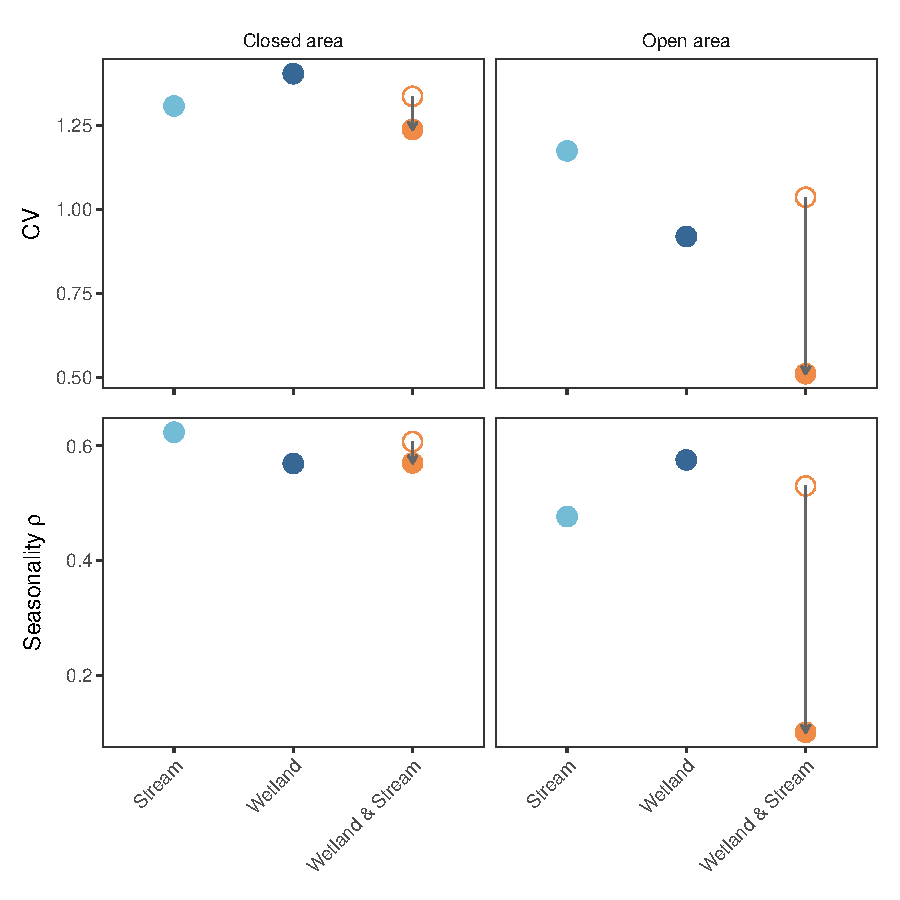
\includegraphics[width=0.6\textwidth]{output/figure_cv_rho.pdf}
    \caption{Wetland-stream complex stabilizes the temporal dynamics of aquatic insect emergence. Panels discern site openness (left column: closed, right column: open) and statistical metrics of temporal dynamics (top row: coefficient of variation [CV], bottom row: seasonality metric $\rho$). Filled circles represent the observed CV or $\rho$ in the respective habitats, while open circles denote the ``predicted'' values of CV or $\rho$, calculated as a weighted mean across stream and wetland habitats. The predicted values reflect expected temporal variability or seasonality under the assumption of perfect synchronization of emergence fluxes across habitats. A reduction in the observed CV or $\rho$ relative to the predicted ones indicates enhanced temporal stability (CV) or reduced seasonality ($\rho$) in resource supply, surpassing what would be expected from a single habitat type alone.}
    \label{fig:cv-emergence}
\end{figure}

\subsection{Temporal Patterns of Bat Activity}

In our dataset, approximately 74\% of recorded bat passes were successfully identified to species. Among these, \textit{E. fuscus} was the dominant species in both open and closed areas, followed by either \textit{N. humeralis} or \textit{L. borealis} (Table S1).
Together, these species comprised the majority of bat passes identified to species.

Our analysis revealed that both site openness and restoration significantly influenced bat activity, with a significant interaction (Table \ref{tab:gam-est}).
The positive influence of site openness aligns with higher bat activity levels observed in the open area, with activity peaking in summer, especially around June, across both restored (wetland and stream) and control sites (stream only) (Figure \ref{fig:bat-activity}).
Notably, the restored site exhibited a prolonged period of high bat activity, which corresponds to the extended emergence window of aquatic insects driven by phenological asynchrony between stream and wetland habitats (Figure \ref{fig:insect-phenology}).

In contrast, temporal patterns of bat activity in the closed area differed significantly from those in the open area, as indicated by the interactive effect of site openness and restoration (Table \ref{tab:gam-est}).
Bat activity was considerably lower in the closed area, with no substantial differences between restored and control sites (Figure \ref{fig:bat-activity}).
These findings highlight the context-dependence of restoration effects.

\begin{table}[ht]
\centering
\caption{Estimated effects of linear predictors in the generalized additive model (GAM).
             Wald p-values were calculated using z-scores derived from the slope estimates and their standard errors (SE).} 
\label{tab:gam-est}
\begingroup\small
\begin{tabular}{lccc}
  \hline
Variable & Estimate & SE & P value \\ 
  \hline
Intercept & $2.64$ & 0.11 & $<0.001$ \\ 
  Restoration (wetland + stream vs. stream only) & $-0.59$ & 0.15 & $<0.001$ \\ 
  Openness (open vs. closed) & $2.22$ & 0.15 & $<0.001$ \\ 
  Restoration $\times$ Openness & $1.12$ & 0.21 & $<0.001$ \\ 
   \hline
\end{tabular}
\endgroup
\end{table}


Importantly, these effects of the linear predictors remain significant after adjusting for seasonality through smoothing terms in our GAM (see Methods).
This confirms that our results are not confounded by seasonal variations in bat activity.

\begin{figure}
    \centering
    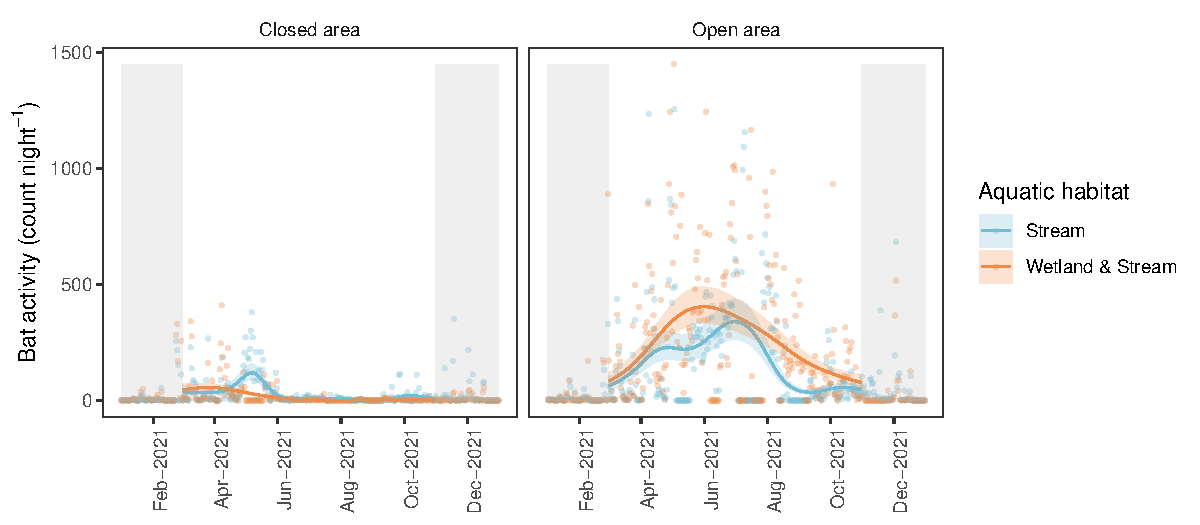
\includegraphics[width=0.95\textwidth]{output/figure_bat_habitat.pdf}
    \caption{Bat activity increased at the restored sites (orange; wetland + stream) relative to the control sites (blue; stream only), but this enhancement was dependent on site openness (panel). Dots represent the observed counts of bat detections, while the lines indicate the predicted values from the generalized additive model, along with their associated standard errors. The shade denotes the period that was not used for our analysis (before March 1 and after October 31).}
    \label{fig:bat-activity}
\end{figure}

\newpage

\section{Discussion}

Habitat loss is a primary driver of biodiversity decline worldwide \citep{chase_ecosystem_2020, fluet-chouinard_extensive_2023}.
As such, restoring degraded or lost habitats, especially in urban areas, is essential for biodiversity conservation and the provisioning of ecosystem services \citep{elmqvist_benefits_2015, palmer_ecological_2014}.
Previous studies indicate that habitat restoration can improve trophic connections across ecosystems through spatial subsidies \citep{buckner_conserving_2018, kupilas_stable_2020}.
However, how restored habitats, such as wetlands, interact with remnant natural habitats to support cross-ecosystem trophic links has remained unclear.
In this study, we found that constructed wetlands complemented remnant urban streams by providing spatial subsidies (emerging aquatic insects) asynchronously, significantly extending the foraging window for terrestrial consumers like bats.
This effect, however, was highly dependent on site openness, underscoring the importance of spatial design in restoration projects \citep{olds_synergistic_2012, gilby_spatial_2018, wahl_approximation_2024}.

The asynchronous emergence of aquatic insects may result from different thermal regimes between aquatic habitats.
Water temperature plays a significant role in the emergence timing of aquatic insects, with warmer temperatures during the growth period promoting earlier emergence \citep{woods_phenology_2022}.
In our study streams, winter water temperatures were higher than in constructed wetlands, though this trend reversed in the summer months (Figure S1).
The accelerated growth of aquatic insect larvae during the winter likely facilitated earlier emergence as winged adults in streams.

The taxonomic composition may also contribute to the distinct emergence phenology between wetlands and streams because emergence timing differs among insect taxa \citep{terui_species-specific_2017, moore_spawning_2010}.
In our data, Diptera dominated in wetlands, whereas both Trichoptera and Diptera were prominent in streams.
Trichoptera emerged from spring to early summer, partially contributing to an earlier and asynchronous emergence peak in streams.
However, it is likely that aquatic insect communities differ substantially at finer taxonomic resolutions (e.g., genus or species) between habitat types.
This variation may be critical to explaining differences in emergence phenology, as closely related insect species can have distinct emergence timings \citep{moore_spawning_2010}.
In our study area, Diptera from streams and wetlands exhibited markedly different phenological patterns despite belonging to the same order (Figure \ref{fig:insect-phenology}).
Unfortunately, further decomposing compositional influences on emergence phenology was not possible as we identified aquatic insects only to the order level.
Addressing this limitation in future studies could reveal how taxonomic differences drive phenological distinctions between aquatic habitats.

The increased bat activity at the restored sites may be an aggregative response to the extended foraging window of emerging insects because the dominant bat species in our study area (\textit{E. fuscus}, \textit{L. borealis}, and \textit{N. humeralis}) are insectivorous and prey on aquatic insects \citep{whitaker_food_1992, clare_species_2009, agosta_habitat_2002}.
Increased bat activities near the water bodies have been found in other species and regions \citep{akasaka_influence_2009, stahlschmidt_constructed_2012, sirami_artificial_2013}, suggesting the broad importance of aquatic insects as food resources.
However, the effect was significant only when the constructed wetland was located in the open area, as observed in some previous studies \citep{stahlschmidt_constructed_2012, sirami_artificial_2013}.
Open areas likely offer easier access to flying aquatic and terrestrial insects, which may enhance foraging efficiency.
In contrast, closed areas with dense canopy structures may impede bat maneuverability, making foraging more challenging.
Thus, the improvement of cross-ecosystem trophic links appears to be strongly influenced by the surrounding habitat structure \citep{marczak_meta-analysis_2007}, highlighting the importance of considering the physical landscape around aquatic habitats in habitat restoration planning.

However, the context-dependent effect of wetland restoration should be interpreted carefully because the observed influence of canopy openness on bat activity may be confounded with other environmental factors.
This research was conducted at one pair of closed and open areas, limiting our ability to statistically distinguish the effect of canopy openness from other confounding factors.
Replicated data of closed-open site pairs are warranted to draw robust conclusions on the influence of canopy openness on the synergies of remnant and restored aquatic habitats. 

Distinct aquatic habitats, or heterogeneous habitats more broadly, provide unique abiotic and biotic conditions that, when combined, enhance ecological stability and resilience as a whole \citep{schindler_population_2010, terui_metapopulation_2018, thorson_spatial_2018, terui_emergent_2021, pomeranz_ecosystem_2023}.
In particular, recent studies suggest the conservation value of phenological diversity emerging from heterogeneous habitats as it underpins a spatial portfolio of critical resources under a changing environment \citep{anderson_portfolio_2015, armstrong_watershed_2020}.
Our study applied the concept of a spatial portfolio to ecological restoration, using the complementary roles of constructed wetlands and remnant streams in providing spatial subsidies as an example.
Our findings emphasize the importance of designing ecological restoration to facilitate the benefit of a heterogeneous landscape.

We acknowledge that generalizing our results to other restoration projects is challenging due to our research being conducted in a restricted area with a single-year dataset.
Nonetheless, we anticipate that synergies between restored and remnant habitats are common, given the growing evidence highlighting the importance of habitat heterogeneity in enhancing ecological resilience.
We hypothesize that asynchronous supplies of spatial subsidies from various donor habitats are particularly important in temporal and boreal biomes due to the clear seasonality.
For example, it has been shown that the emergence of aquatic insects has sharp seasonal peaks in temperate and boreal biomes, whereas a tropical biome lacks such seasonal patterns \citep{nash_latitudinal_2023}. 
Further studies that extend our findings to other regions or ecosystems may yield deeper insights and help increase our ability to conserve ecosystems.

% \section*{Acknowledgements}
% We thank many undergraduate and graduate students who helped with our fieldwork.
% This work is based on the materials supported by startup funds (to AT) and the Undergraduate Research and Creativity Awards (to MI) at the University of North Carolina at Greensboro.

% \section*{Conflict of Interest}

% None declared.

% \section*{Data availability}

% Data and codes will be available at \url{https://github.com/mni1220/public-proj_uncg_wetland} upon acceptance.

% \section*{Author Contributions}

% AT conceived the research project.
% MI, RP, CFW, and AT collected data, and MI performed data analysis with inputs from AT and RP.
% MI wrote the first draft, and all authors contributed significantly to the conception and improvement of the manuscript. 

\newpage

\bibliography{tex/references, tex/ref_package}

\end{document}